\section{Probability ve Likelihood}
Türkçede ikiside olasılık olarak çevilirilir. Fakat istatistikte farklı anlamlar taşırlar. Probability, gelecekteki bir olayın gerçekleşme olasılığını ifade eder. Bir olayın olasılığı, önceden belirlenmiş belirli bir örnek uzayına göre hesaplanır. Formülü P(A) = n(A) / n(S). Likelihood bir olayın gözlemlenen verilere göre ne kadar olası olduğunu ifade eder. Verilerden sonra hesaplanır. Likelihood bir sonuçtur. Formülü $L(D | \theta) = f(D | \theta)$.

\begin{figure}[h]
    \centering
    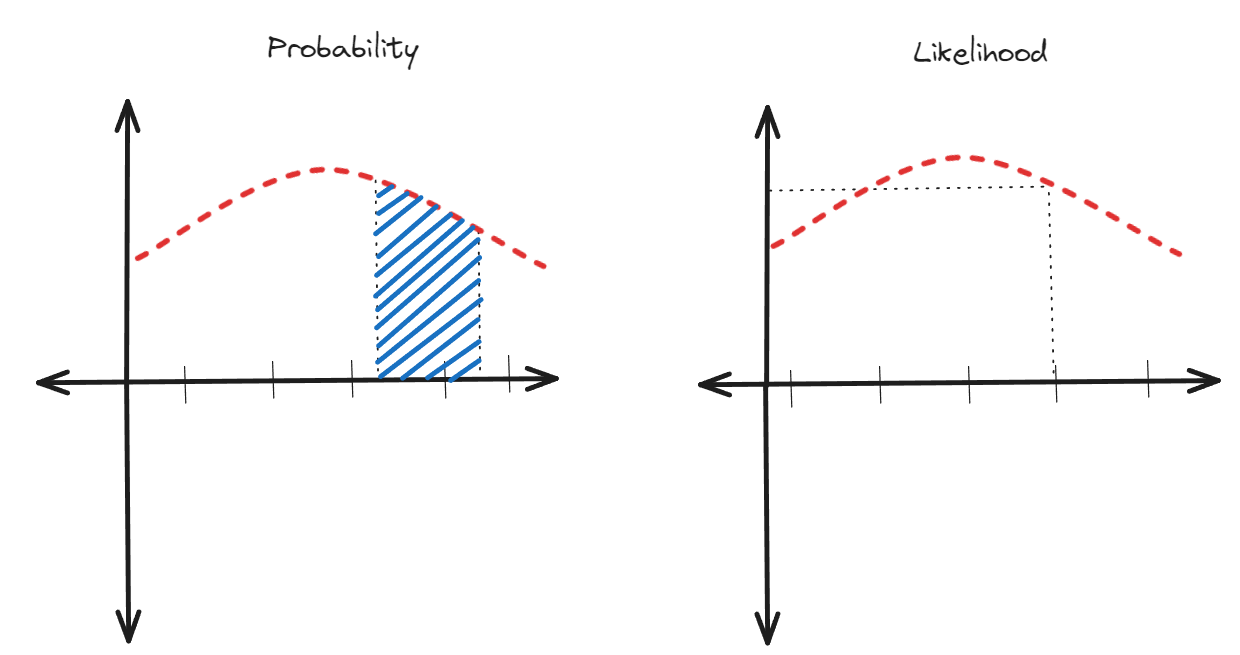
\includegraphics[width=1\textwidth]{images/probability_vs_likelihood.png}
    \caption{Probability vs Likelihood.}
    \label{fig:enter-label}
\end{figure}

Bir madeni paranın yazı gelme olasılığı 0.5'tir. Bu bir olasılık değeridir. Ancak madeni parayı 10 kez attığımızı ve 8 kez yazı geldiğini varsayalım. Bu durumda yazı gelme likelihood'u $\frac{2^8}{2^(10)}$'dan 0.25'tir. Bu değer, gözlemlenen veriler göz önüne alındığında yazı gelme olasılığını gösterir.

\newpage